% !TEX root = tese.tex


\chapter*{Introdução}
\addcontentsline{toc}{chapter}{Introdução}
\label{ch:intro}

Esta pesquisa tem vários pontos de partida. Como um projeto transdisciplinar, entre campos como Música, Design e Computação Musical, parte de uma pesquisa anterior de investigação das tecnologias que dão suporte à web, desde o trabalho final de graduação na Faculdade de Arquitetura e Urbanismo da Universidade de São Paulo (FAU), um dicionário de linguagens de marcação e programação para web (HTML, CSS e JavaScript), que continuou no mestrado\footnote{Com a dissertação ``World Wide Web: Forma aparente e forma oculta'', procurei investigar história, processos e metodologias para o design de websites, com o sentido de aproximar os campos de atuação de designers e programadores}. Parte também de uma prática de produção, edição e gravação experimental de música e do trabalho junto a diversos grupos e coletivos em  práticas artísticas diversas, parte delas organizadas no acervo da página Finetanks.com que mantenho desde 2005.  
    Esta tese, surge em parte como um desejo de síntese entre essas diversas práticas e interesses, no campo do design, programação e música, de um desejo de investigar os potenciais de exploração de tecnologias web para criação musical. 
    
    
    Filósofos da sociedade pós-industrial como Daniel Bell (1979) \footnote{\cite{bell1979thinking}} relacionam o processo de digitalização da informação e dos meios de comunicação com a emergência de uma sociedade pós-industrial, onde a ``a informação se tornou o recurso estratégico e transformador na sociedade como o trabalho e o capital foram recursos estratégicos e transformadores na sociedade industrial'' \footnote{\cite[26]{bell1979thinking}}. Neste contexto, os sistemas de comunicação se tornam a principal estrutura de amarração e unificação da sociedade. Bell, que Richard Barbrook \footnote{\cite{barbrook1999cyber}} considera um dos principais expoentes da esquerda estadunidense da guerra fria, já apontava as potencialidades da criação de uma rede mundial de computadores como catalisador de interações interpessoais e como ampliadora das ``arenas onde ocorrem as ações sociais" \footnote{\cite[22]{bell1979thinking}}. Bell, desenvolve essa noção de ``sociedade da informação'' a partir de idéias propostas por Marshall McLuhan, difundidas principalmente no livro ``Os meios de comunicação como extensões do homem''\footnote{\cite{luhan1964marshall}}, de que a sociedade se  transforma a cada mudança ocorrida nas tecnologias e nos meios de comunicação. 
    
    A internet pode ser considerada uma espécie de ``meio de meios'' \footnote{\cite[5]{Levinson2001}}, que começou como um sistema de troca de informação, onde imperava principalmente o texto e passou gradualmente a ser suporte para diversos outros  meios de comunicação como telefone, rádio, cinema e televisão, um meta-meio, cujo conteúdo é, não só o conteúdo de todos meios anteriores, mas também o próprio usuário que coloca o conteúdo online \footnote{\cite[39]{Levinson2001}}. Quando Levinson analisava McLuhan em ``Digital McLuhan'', a internet ainda era um meio ainda dominado principalmente pela tecnologia da escrita, e sendo assim, dominado ainda pelo espaço visual. Apesar disso, a música foi um dos conteúdo significativos da rede, desde os primeiros sistemas de de compartilhamento de arquivos entre usuários, e o desenvolvimento constante das tecnologias, traz a ela cada vez mais novos potenciais acústicos.
    
Hoje, por exemplo enquanto escrevo esse texto, posso ouvir qualquer estação de rádio do mundo que faça \emph{live streaming} pela internet, através de um site como o Radio.garden (figura \ref{radiogarden}), por exemplo. O projeto coordenado pelo Netherlands Institute for Sound and Vision, reúne as estações de rádio em um mapa, e podemos acessá-las de qualquer lugar, e trocá-las com um girar do globo com o mouse, permitindo aos ouvintes a conexão com culturas distantes, ao explorar formas diversas de transmissão e identidades culturais de todo planeta \footnote{\cite{caroline2016radio}}. 

\begin{figure}[htb]
    \caption{\label{radiogarden} Radio.garden.}
    \begin{center}
        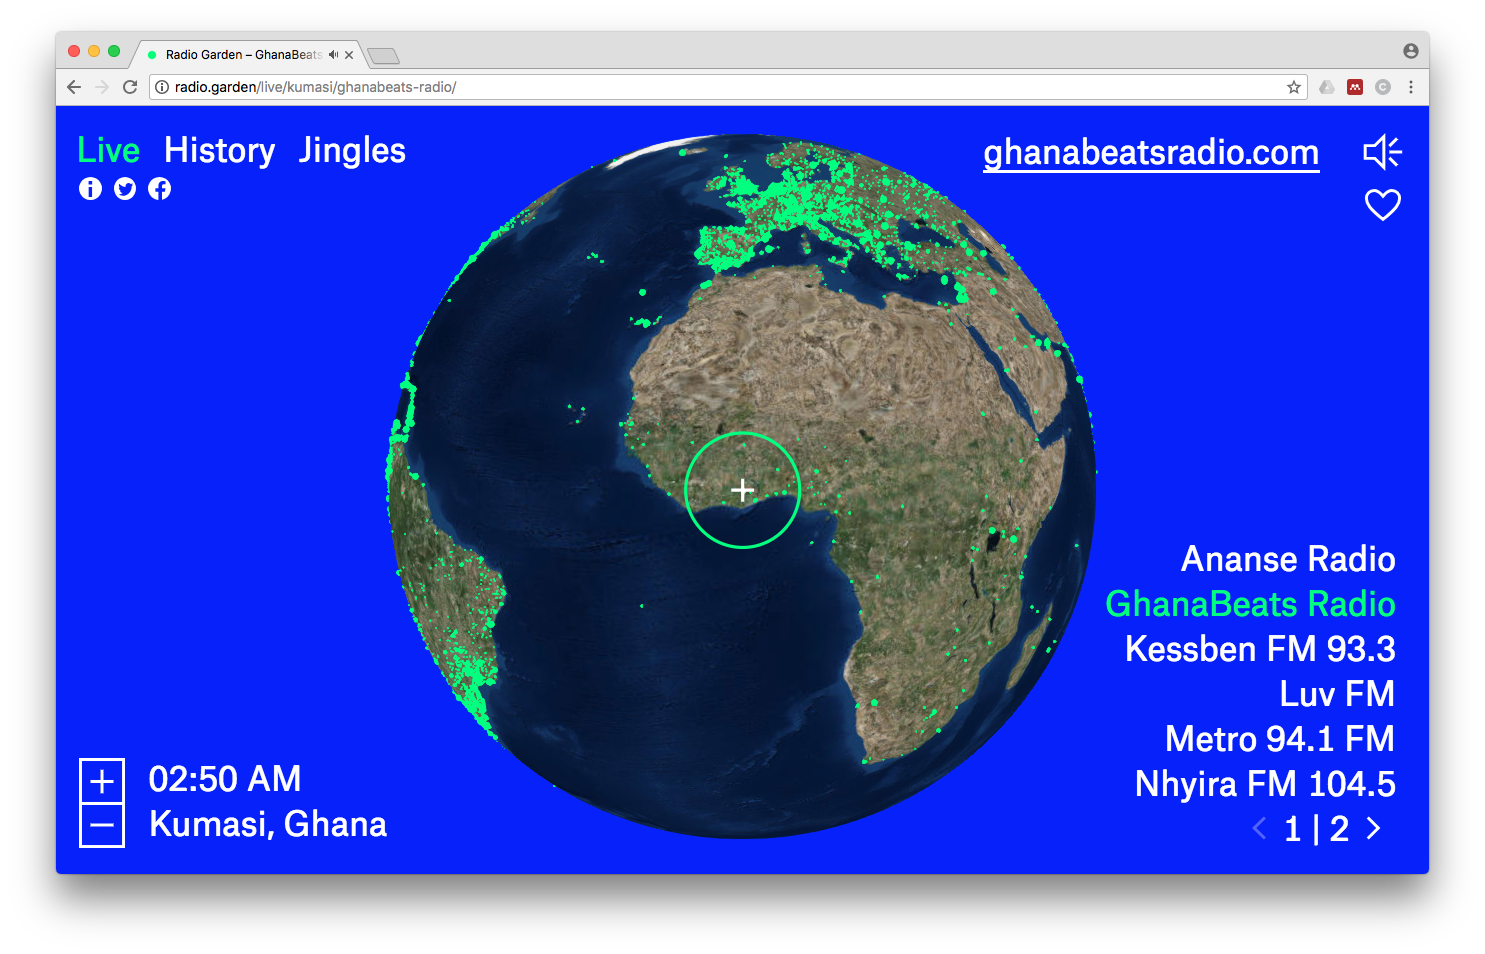
\includegraphics[width=1\linewidth]{pictures/radio_garden_2018-06-10.png}
    \end{center}
    \legend{Fonte: Screenshot da autora, 8 de junho de 2018}
    
\end{figure}
%\legend{Fonte: \citeonline[p. 24]{araujo2012}}

Posso também acessar uma base de dados extensiva da produção humana em música, cinema e televisão construída a partir do trabalho de pessoas em todo o planeta, reunida em grandes portais como o Youtube, onde segundo estatísticas atuais são depositadas 300 horas de conteúdo a cada minuto. Mas, como bem apontou a compositora Pauline Oliveros em ``Software for people", ``As mídias e a maior mobilidade obviamente acomodam mais informação, mas não necessariamente mais sabedoria"\footnote{\cite[179]{Oliveros2012}}. 

Teóricos da sociedade da informação, professavam que a internet teria um papel demiúrgico, que ``libertaria a humanidade sem qualquer necessidade de luta de classes" \footnote{\cite[275]{Barbrook2009}}. Para Howard Rheingold, da revista Wired, por exemplo, a internet também seria a ``curandeira da alientação social'', como aponta Barbrook:


\begin{citacao}
Em sua atualização da Nova Esquerda mcluhanista do início dos anos 1990, BBSs, MUDs, NT2, serviços de bate-papo instantâneos e servidores de lista de e-mail representavam os princípios da ágora eletrônica postos em prática: as “comunidades virtuais”. Fundada sobre o compartilhamento de informação e conhecimento, a Internet era uma das “ferramentas para pensar” que liberariam a humanidade da sociedade fabril fordista. \footnote{\cite[350]{Barbrook2009}}
\end{citacao}

Mas sob a neoliberal ``ideologia californiana'', a internet se transformou na apoteose do mercado \footnote{(idem, p. 353)}. Em ``Technologies of Freedom'', de 1983 Ithiel de Sola Pool codificava o que Barbrook chama de ``sua apropriação neoliberal do mluhanismo'':
\begin{citacao}
Ao invés de construir a ágora eletrônica, a convergência da mídia, das telecomunicações e da computação criava o mercado eletrônico. De programas de computadores a novelas, todas as formas de informação seriam logo negociadas como mercadorias pela Internet. Pela primeira vez, todos poderiam ser um empreendedor de mídia. \footnote{\cite[348]{Barbrook2009}}
\end{citacao}

Ele apnonta ainda que há quem inclusive culpe a mídia eletrônica por exacerbar uma série de de males da sociedade como: ``elitismo, pedofilia, terrorismo, deficiência educacional e solidão''. 

Não é difícil de concordar com essa visão. Uma simples tecnologia que permite ao usuário deixar sua opinião nas notícias dos grandes portais é suficiente para nos assombrar com o nível de barbárie latente na sociedade, a cada notícia veiculada na supostamente isenta ``grande mídia". Abre espaço para a voz do Zé Ninguém, como definido por Wilhelm Reich \footnote{\cite{reich1998escute}}, aquele ser de mentalidade tacanha, que ``está sempre do lado dos perseguidores'' (p. 27), que persegue mães solteiras, por serem imorais, ao mesmo tempo que cultua Jesus, que ``é tolerante com a sua própria religião mas com nenhuma outra (p.51)":

\begin{citacao}
como não tem memória para coisas que aconteceram há dez ou vinte anos, você ainda repete os mesmos disparates de dois mil anos atrás. Pior, você se agarra com unhas e dentes a absurdos como ``raça'', ``classe'', ``nação'' e à obrigação de seguir uma religião e reprimir sua desgraça. \footnote{\cite[101]{reich1998escute}}
\end{citacao}

No momento em que escrevo esta tese, passamos no Brasil por uma eleição onde o candidato vencedor explorou fortmente o apelo de notícias para uma população desinformada que pode acreditar nos maiores absurdos propagados pelas redes sociais. Produtores de notícias falsas por todo o mundo exploram deliberadamente recursos e algoritmos das redes sociais para propagar suas mensagens \footnote{\cite{Martens2018}}, que influenciam resultados políticos em diversos países.

Apesar disso, nós, que somos artistas, pesquisadores e pessoas que criam, não podemos nos sujeitar passivamente à essa visão apocalíptica de que a internet está nos levando à barbárie, e podemos pensar nos meios tecnológicos como ponto de partida para novas proposições éticas e estéticas. Concordamos com arquiteto e pintor Sérgio Ferro quando afirma: que a expressão humana na arte é ``pegar a necessidade histórica que está no material e trabalhá-la até o fundo", \footnote{\cite{FerroSergio2002}} e que isto é a própria essência da liberdade. Sendo operadores de cultura, não devemos negar a indústria cultural, mas como já apontava Eco (\citeyear{Eco1970}), ``Colocar se em relação dialética, ativa e consciente com os condicionamentos da indústria cultural''\footnote{\cite[14]{Eco1970}}. Para ele, esse é o único caminho possível para que o ``operador de cultura'' cumpra sua função. Para ele, as codições objetivas devem ser o ponto de partida para a nossa criação artística: 



\begin{citacao}
A nosso ver, se devemos operar \emph{em} e \emph{para} um mundo construído na medida humana, essa medida será individuada não adaptando o homem a essas condições de fato mas \emph{a partir dessas condições de fato}. O universo das comunicações de massa é -- reconheçamo-lo ou não -- o nosso universo; e se quisermos falar de valores, as condições objetivas das comunicações são aquelas fornecidas pela existência dos jornais, do rádio, da televisão, da música reproduzida e reproduzível, das novas formas de comunicação visiva e auditiva. Ninguém foge a essas condições, nem mesmo o virtuoso, que, indignado com a natureza inumana desse universo da informação, transmite o próprio protesto através dos canais de comunicação em massa, pelas colunas do grande diário, ou nas páginas do volume em \emph{paperback}, impresso em linotipo e difundido nos quiosques das estações.\footnote{\cite[13]{Eco1970}}

\end{citacao}

 Lev Manovich (\citeyear{Manovich2008}), artista que também teoriza sobre as ``novas mídias'', cunhou o termo ``infoestética'' \footnote{\cite{Manovich2008}}, para se referir às práticas culturais que surjem em resposta às questões da sociedade da informação, tirando sentido, trabalhando com ou produzindo conhecimento a partir da informação, examinando muitos campos culturais onde o emprego da computação deu origem a ``novas formas''. Se nossas condições objetivas nos colocam a realidade da internet e das mídias sociais como os meios de comunicação estruturantes das relações humanas atuais, pensar esses meios criticamente também é uma das tarefas dos artistas e produtores culturais. Em uma sociedade fortemente mediada por tecnologias de computação, a programação pode ser uma forma de potência, que permite ao agente atuar sobre a cultura da informação para além da posição de observador.

\subsection{Música como potência}
Dentre as demais formas de arte, consifero que a música é epecialmente potente. 

%literalmente pode se falar de potência sonora

O som é quase impossível de se bloquear, e sendo assim, a música tem a capacidade de atingir as pessoas circundantes de uma maneira geral e compulsória, uma vez que energia sonora é das mais difíceis de se conter em termos coletivos. É possível um indivíduo tampar seus próprios ouvidos, mas é muito difícil tapar os ouvidos alheios, e mesmo tapando os ouvidos, nunca haverá silêncio\footnote{É famoso o experimento de John Cage que 1951 entrou em uma câmara anecóica, onde supostamente haveria silêncio total. Ao invés de encontrar o silêncio, Cage ouviu os sons do seu sistema nervoro (agudo) e circulatório (\cite{Mauceri1997})}. Levinson (\citeyear{Levinson2001}) aponta que o som tem como característica``emanar de todos ambientes'', e enquanto a visão nos dá detalhes preciso, ponto-a-ponto do ambiente ao nosso redor, é a audição que ``nos mantém em contato com o mundo vinte e quatro horas por dia" \footnote{\cite[47]{Levinson2001}}. No ``Panorama setorial da cultura brasileira'', levantamento feito sob coordenação de Gise Jordão, levantamento 
 

Minha relação com a produção musical teve muita relação com um potencial de agregação que a música traz. Primeiro, como dj, organizando festas que eram essenciais para o financiamento do grêmio dos estudantes da FAU, depois, no Urbando, grupo de maracatu que intervinha também em atos estudantis. Sempre foi muito nítido pra mim o potencial de um tambor ou um xequerê como instrumento de organização de massas em atos, como instrumentos para colocar as pessoas em movimento. Não é atoa que os exércitos usam marchas como forma de elevar a moral dos soldados\footnote{Pauline Oliversos cita em ``Software for People'' (p. 99) que a música militar foi o primeiro tipo de música introduzida no Oriente pelo Ocidente. \cite{Oliveros2012}}, e que também as igrejas usam música para encantar os fiéis. O discurso verbal pode ser cansativo, o texto pode ser ignorado, enquanto a música é capaz de colocar uma multidão em uníssono. Em uma sociedade como a nossa, esse poder é exercido principalmente pela indústria cultural, que afasta esse sentido político que a música pode ter, convertendo tudo em mercadoria, como aponta Marilena Chauí no seu artigo ``Cultura e Democracia'': 

\begin{citacao}

Como cultura de massa, as obras de pensamento e de arte tendem: de expressivas, tornarem-se reprodutivas e repetitivas; de trabalho da criação, tornarem-se eventos para consumo; de experimentação do novo, tornarem-se consagração do consagrado pela moda e pelo consumo; de duradouras, tornarem-se parte do mercado da moda, passageiro, efêmero, sem passado e sem futuro; de formas de conhecimento que desvendam a realidade e instituem relações com o verdadeiro, tornarem-se dissimulação, ilusão falsificadora, publicidade e propaganda. mais do que isso. A chamada cultura de massa se apropria das obras culturais para consumi-las, devorá-las, destruí-las, nulificá-las em simulacros. Justamente porque o espetáculo se torna simulacro e o simulacro se põe como entretenimento, os meios de comunicação de massa transformam tudo em entretenimento (guerras, genocídios, greves, festas, cerimônias religiosas, tragédias, políticas, catástrofes naturais e das cidades, obras de arte, obras de pensamento). É isto o mercado cultural. \footnote{\cite[61]{MarilenaChaui2008}}
\end{citacao}

Uma cultura democrática, seria aquela, segundo ela, onde as pessoas tenham acesso aos meios de produção cultural, e não somente aos produtos de seu mercado. Tendo uma formação em arquitetura e design, e sendo assim de certo modo estranha ao contexto e aos códigos da música tradicional, foi fácil notar o alto grau de fechamento da cena musical, especialmente para mulheres, como aponta Pauline Oliveros no texto ``And don't call them Lady Composers" \footnote{\cite[48]{Oliveros2012}}. 

\subsection{Acesso}
Uma das coisas que colabora com esse hermetismo é a dificuldade de acesso aos instrumentos musicais, que podem ser muito caros, pesados ou de difícil manipulação. O acesso aos meios de produção certamente é uma das barreiras que afasta as pessoas de uma vivência musical cotidiana. Instrumentos musicais, equipamentos de áudio em geral e controladores, podem ser muito caros, complexos e de difícil manipulação\footnote{\cite{Fiebrink2007}}. A digitalização das tecnologias de produção musical, no entanto, tornou acessível aos usuários de computadores pessoais, tecnologias que só eram disponíveis para grandes estúdios musicais. A partir dos anos 80, isso causou um crescimento exponencial do engajamento da juventude com meios de produção musical digitais, como aponta Georgina Born \footnote{\cite[143]{Born2015}}, mas também causa a uma ``tecnofilia fetichista'' em relação a equipamentos e tecnologias \footnote{(idem, p. 145)}.

Como aponta Baudrillard em ``O sistema de objetos", ``os consumidores não têm acesso à igualdade diante do objeto depois da Revolução Industrial" \footnote{\cite[162]{Baudrillard2012}}. Podemos dizer que a revolução digital, tem permitido concentrar uma série de funcionalidades em gadgets como celulares ou laptops, cada vez menores e mais complexos, que exercem cada vez mais uma dominação dos sentidos individuais das pessoas – que ficam dependentes e absortas em complexas tramas de dados e dramas. O gadget para Baudrillard é um objeto que faz parte de um universo de delírio funcional, um tecnicismo excêntrico e formalismo gratuito, objetos tomados totalmente pelo imaginário, ou obsessões pura e simples, aberrações funcionais. \footnote{(idem p.121)}. 

Meu projeto parte de um desejo de libertação dessa dependência de toda uma uma parafernália tecnológica, concentrando esforços em desenvolver protótipos experimentais para produção musical em tecnologias para a rede, que possam ser acessadas pelas pessoas de seus aparelhos de uso cotidiano: computadores pessoais, aparelhos de celular. Soluções deste tipo poderiam ser mais acessíveis, já que um instrumento musical online poderia ser acessado por qualquer dispositivo que tenha acesso à internet -- gadgets que ganharam muito poder de processamento, nos quais já estamos absortos. 

Dessa forma, essa pesquisa se insere também em um campo que tem se configurado recentemete como Música Ubíqua, que segundo Keller (\citeyear{Keller2018}), tem como objetivo prover acesso à tecnologias para prática musical a um número maior de pessoas, ou ``uma nova maneira de promover a criação musical em contextos não antes acessíveis a empenhos artísticos''\footnote{\cite{Keller2018}}. Para isso, pesquisadores do campo tem investigado o uso de tecnologias web e o do uso de dispositivos móveis, como celulares para produção musical. 

 Além disso, tinha um desejo sobretudo de investigar novas formas de interface, por considerar que muitas das interfaces existentes, que são em maioria baseadas nas de equipamentos eletrônicos \footnote{\cite{Stolfi2016}}, também exigem a necessidade de saberes bastante específicos em tecnologias musicais, além de imporem certos parâmetros da música tradicional, como notas, timbres e tempos. 

Com o desenvolvimento da pesquisa, e o meu contínuo envolvimento com práticas musicais como a da improvisação livre, ``uma pragmática musical aberta à variação infinita em que os sistemas e as linguagens deixam de impor suas gramáticas abstratas e se renderem a um fazer fecundo" \footnote{\cite[2]{Costa2016}} esse desejo de construção de instrumentos genéricos foi se direcionando para a construção de instrumentos específicos para suprir necessidades pessoais musicais -- como é o caso do projeto Banda Aberta e o Playsound.space, projetos que desenvolvi nesta pesquisa e que descreverei mais à frente nesta tese -- sempre buscando portabilidade e facilidade de uso.


Além da questnao da materialidade dos intrumentos físicos, o acesso à prática musical também passa pela questão do domínio do ``gesto musical''. Na música tradicional, o gesto -- do performer ou do intérprete -- é tradicionalmente o gerador do som. O domínio do ato de tocar, principalmente instrumentos tradicionais, envolve um domínio de uma linguagem corporal que gera o som desejado de acordo com o desejo do musicista. Na música instrumental e vocal, sempre há um gesto físico que gera o som, o que não acontece necessariamente na música eletrônica \footnote{\cite[85]{Smalley1996}}. Isto é uma preocupação de quem desenvolve aplicativos para música interativa, como aponta Schnell (\citeyear{Schnell2013}): 


\begin{citacao}
Two principal concerns constitute the design of interactive audio applications and musical instruments of virtually any kind. One deals with creating real-time interactive sound processes and the other with the way these sound processes are influenced by the bodily movements and gestures of their players. In this sense, the essence of designing interactive audio applications lies in the creation of meaningful relationships between movement – or gestures – and sound. \footnote{\cite{Schnell2013}}
\end{citacao}
Essa questão também é discutida no âmbito das \emph{laptop orchestras}, como aponta Trueman (2007):
\begin{citacao}
Para a performer de \emph{laptop}, isso parece representar um grande problema. Se parecer que nós estamos simplesmente respondendo e-mail equanto geramos sons, o que que o ``ouvinte'' vai pensar de tudo? que tipo de performance sofrível que isso poderia possivelmente inspirar? Como pareceria uma dancinha de computadores no ar\footnote{Aqui uma referência a \emp{air-guitar}, quando se imita o gesto de um guitarrista}?
Mas talvez isso seja uma oportunidade ao invés de um problema, um desafio para o qual a orquestra de laptops é um ginásio socialmente carregado. Por um lado, nós podemos encarar de frente e se esforçar para criar instrumentos desafiadores que podem gerar sons que pareçam de certa forma tangíveis (mesmo acústicamente), relacionados à fisicalidade que eles exijam.\footnote{\cite[6]{Trueman2007}} 
%For the laptop performer, this seems to pose a
%deep problem. If we look like we are simply doing e-mail while generating sounds that provoke the motor-mimetic response of, say, striking an enormous hammer, what will the ‘listener’ make of it all? What kind of vicarious performance could this possibly inspire?What would the ‘air-laptop’ dance look like? 
%But perhaps this is an opportunity instead of a problem, a challenge for which the laptop orchestra is a musically and socially charged gymnasium. On the one hand, we can go at it head-on and endeavour to create challenging instruments that generate sounds which somehow seem tangibly (even acoustically) related to the physicality they demand.
\end{citacao}

A noção de virtuosidade, para Smalley ({\citeyear{Smalley1996}) é baseada na identificação de um controle consumado na articulação de morfologias sonoras. No seu modelo do espectro de sons, Smalley considera como sons musicais, aqueles gerados com intenção pelos homens. Mesmo sons naturais podem ser convertidos em música, desde que sejam resultado de uma agência humana. O campo da música eletroacústica foi responsável por inserir na música uma ampla gama de sons sintetizados e da natureza que não necessariamente podem nem ter tido uma existência material. Muitos trabalhos acusmáticos, inclusive, não possuem nenhuma fonte sonora gestual visível em tempo real\footnote{\cite[95, 101]{Smalley1996}}, como no caso acima mencionado, das orquestras de laptops. Mas mediação dos processos musicais pelo computador vai muito além, no entanto, desse âmbito; desde o processo de composição ao de difusão musical. Para produção musical, por exemplo, existem hoje muitos tipos diferentes de software. Hugill \citeyear{Hugill2012} cita por exemplo: gravação, edição e sequenciamento; processamento de sinais; samplers; instrumentos virtuais (vst); sintetizadores; performance ao vivo; notação; composição; análise e representação e modulares ou construíveis\footnote{\cite[195]{Hugill2012}.

%\begin{citacao}
%Music production relies on software. To specify precisely which music software packages might be useful to the musician is futile, because the software market changes so rapidly. However, it is possible to identify generic types of music software, as follows:
%• software para gravação , edição e sequenciamento de sons • aplicativos para processamento (incluindo \emp{plugins}) • software de sampleamento • instrumentos virtuais • softwares para síntese • software para performance ao vivo • software para notação • software para composição • software para análises ou representação • softwares modulares ou do tipo faça você mesmo., tradução nossa}
%\end{citacao}

Não se pode ``fazer muito sem software em música nos dias de hoje'', como aponta Miller Puckette \citeyear{PucketteMiller}, que é músico improvisador e também desenvolvedor do Pure Data. Isso cria uma relação de inter-dependência entre os usuários e os desenvolvedores de software, que ``são dependentes dos ``usuários'' (os músicistas) para fazer atividades artísticas com seus softwares; sem isso, o trabalho de desenvolvimento de software é sem sentido''. Tanto Hugill \citeyear{Hugill2012} como Puckette \citeyear{PucketteMiller} apontam também que o software influiencia diretamente o trabalho dos artistas, oferecendo constrições, direções ``até mesmo em direção a um gênero ou estilo específico''\footnote{\cite[195]{Hugill2012}}. 

%Músicistas não conseguem fazer muita coisa hoje em dia sem software, e sendo assim eles são dependentes dos desenovedores de software. Desenvolvedores de software, por sua vez, 

%The digital musician will need to be aware that such software can try to steer musical content in a particular direction, even towards a specific genre or style. Sometimes music production is a matter of finding ways to achieve something original in spite of the software design. \footnote{\cite[195]{Hugill2012}}

%\end{citacao}

Nessa pesquisa, os papéis de desenvolvedor e usuário se misturam, uma vez que estamos desenvolvendo ferramentas que sirvam acima de tudo para o nosso próprio trabalho. Nos amparamos um tanto pela a ética do \emph{hacker}, no sentido que aponta Giuliano Obici, tendo ``a paixão pelo fazer como uma busca exploratória'' que ``que se fundamentam pela liberdade, criatividade aberta ao jogo e à experimentação''\cite[366]{Obici2014}, mas também um pouco tanto de \emph{bricoleur}, que segundo ele:
\begin{citacao}
Ao mesmo tempo, o  se difere do engenheiro por seu conjunto de meios não se basear em um projeto, seguindo o princípio de que “algo sempre pode servir para algo”, sua instrumentalidade parte de elementos recolhidos e/ou achados. Sem um planejamento preconcebido, afastado dos processos e normas adotados pelo pensamento técnico instrumental, o bricoleur se vale de materiais fragmentários pré-elaborados. \cite[366]{Obici2014}
\end{citacao}

Algumas vezes, quando começamos um projeto, não tínhamos uma ideia total de qual seria o resultado final. Muito das metodologias utilizadas foi sendo agregado durante o processo, como por exemplo as avaliações com usuários ou análises estatísticas, que são coisas que não eram previstas inicialmente, mas que no processo de produção e desenvolvimento e publicação dos resultados, passaram a fazer sentido de serem testadas. Nos próximos capítulos apresentaremos uma síntese do percurso que me levou a essa pesquisa, a partir da relação entre música e rede; em seguida, apresentamos um momento inicial do trabalho onde buscamos referências históricas e contemporâneas para essa pesquisa; no terceiro capítulo apresentamos os primeiros exoercícios e resultados obtidos, até o projeto de performance participativa Banda Aberta; o quarto capítulo é dedicado ao Playsound, que é um instrumento online para tocar com sons concretos, especialmente em contextos de improvisão livre, baseado na biblioteca de sons em licensas livres Freesound.org; por fim, aprensentamos algumas conclusões deste processo, que também geram indagações para a continuação de uma pesquisa que não se encerra nessa tese.






%\todo[inline]{a partir daqui precisa reescrever e reposicionar tudo}





%\subsection{Cultura Livre}

%Procuramos defender uma idéia de cultura livre, que permeia uma série de práticas, desde a escolha das linguagens, do repertório e dos projetos, até a publicação de código aberto e conteúdo em licenças livres. A própria adoção de práticas de improvisação livre tem relação com essa idéia. A digitalização da arte leva à possibilidade de livre reprodução, e amplia sua sua exponibilidade, como já apontava Benjamin (1987). A própria web foi construída com base em idéia de livre circulação da informação, na adoção de uma estrutura não hierárquica e de linguagens livres de marcação (Berners-lee, 1989).





%\subsection{Brutalismo Digital}
%É importante notar, mesmo que brevemente, algumas referências  estéticas, e especialmente da influência da arquitetura moderna e do brutalismo de Vilanova Artigas e da precariedade radical de Lina Bo Bardi, dos concretistas russos como El Lissitsky e Rodchenko e brasileiros como Sacilotto, Athos Bulcão e Lygia Pape, Erthos Albino de Souza, Augusto de Campos, Haroldo de Campos e Décio Pignatari. 

%Trabalhar a partir de  referências do passado pode trazer certas questões ideológicas, como aponta Plaza (idem, p. 6):

%\begin{citacao}
%Operar sobre o passado encerra um problema de valor. Não é escolher um dado do passado, uma referência passada; é uma referência a uma situação passada de forma que seja capaz de resolver um problema presente e tenha afinidade com suas necessidades precisas e concretas, de modo a projetar o presente sobre o futuro. Toda época distingue entre formas conservadoras e mais inovadoras. As inovadoras são as que se projetam para o futuro através do caráter inacabado que aponta para um possível leitor, o que é também uma forma de ``perceber na cultura de hoje os traços reais e inconfundíveis do amanhã''. Operar sobre o passado, além de um problema de valor, constitui-se também numa operação ideológica através da qual podemos confirmar a produção do presente ou encobrir essa realidade. Se, no primeiro caso se favorece um encontro dialético com o passado para preparar o futuro, no segundo, trata-se de distanciar esse futuro indefinidamente. No primeiro caso, os valores da história constituem-se num modelo para a ação, já no segundo, trata-se de um fantasma a ser evocado como nostalgia, moda ou revival. \footnote{\cite{JulioPlaza1969}}
%\end{citacao}

%Aqui, não queremos trazer essas referências como inspiração ou nostalgia, mas como apontamentos para pensar possibilidades estéticas. Como os princípios de racionalidade,  e sobretudo uma postura anti-decorativa, anti-ornamental e de procurar um mínimo de elementos necessários.

%\subsection{Trans-disciplinaridade}


%\subsection{Antropofagia}

    % Write epigraphs
    

 %\begin{citacao}
%Na arquitetura aberta da Internet, as restrições da propriedade intelectual tornavam-se um anacronismo. Embora produtores ainda pudessem impedir que seu trabalho fosse apropriado por outros, todos deveriam ser autorizados a copiar e alterar informações para seus próprios propósitos. Em meados dos anos 1990, Stallman lançou uma campanha para as leis de propriedade intelectual dos Estados Unidos serem reformadas de acordo com o método de trabalho ao estilo universitário: “copyleft” \footnote{\cite[368]{Barbrook2009}} \citeyear{Barbrook2009}
%\end{citacao}


%Neste capítulo procurarei tratar especificamente desta influência, bem como da de artistas que tomaram esse princípio para suas práticas, como Lygia Clark e Hélio Oiticica, neste que tem um certo aspecto de devoração do outro e um sentido de busca de alegria e liberdade, 

%relacionando também com práticas correntes junto a redes como a do tecnoxamanismo, que trouxeram novas perspectivas neste sentido.


%\begin{citacao}
























    \newpage
